\section*{ \sloppy \center Добавление.Оптимальное распределение плотности источников тепла }
\sloppy
\emergencystretch=20pt


 Рассмотренные выше прямые методы вариационного исчисления не исчерпывают всех возможных методов численного решения бесконечномерных задач.
Существует ряд прикладных задач, при решении которых приходится комбинировать известные методы или изобретать новые.

Одной из инженерных задач, связанных с ресурсосберегающими технологиями, является задача об оптимальном расположении источников тепловых полей. Она всегда была актуальной задачей при проектировании в строительстве, металлургии и других областях техники. Эта задача допускает ряд постановок, которые не эквивалентны из-за различий в критериях оптимизации. По сути, здесь мы имеем целый ряд задач. Они различаются как по постановке, так и по методам решения. В настоящем разделе в качестве примера бесконечномерной задачи оптимизации рассматривается задача нахождения плотности источников тепла минимальной суммарной интенсивности, которая обеспечивает приемлемое распределение температур в области, находящейся в состоянии стационарного теплового баланса с окружающей средой. Умение решать такую задачу может быть использовано при оптимальной организации обогрева жилых и производственных помещений, для поддержания заданного температурного режима в однородных и неоднородных твердых телах и т.д. Перед тем, как дать точную формулировку задачи, сделаем несколько замечаний.

Существует три основных механизма распространения тепла: теплопроводность, конвекция и излучение. Последний играет существенную роль при высоких температурах (порядка $500-600^0 $), поэтому в упомянутом выше круге задач этот механизм можно не учитывать. Чрезвычайно сложным является учет свободной конвекции, возникающей в гравитационном поле. Поскольку мы рассматриваем стационарные тепловые процессы, в которых свободная конвекция может
 отсутствовать\footnote{  При определенных условиях могут возникать стационарные конвективные течения. В рассматриваемых здесь работах их влияние считается несущественным.}, ее мы тоже не учитываем.

В итоге, как указано ниже, получается задача оптимального управления для эллиптических краевых задач. Вообще говоря, точного решения этой задачи может не существовать. Поэтому мы уточняем постановку задачи, вводя так называемое \textit{квазирешение} или
 \textit{$\varepsilon$-оптимальное решение}
Далее кратко излагается методика численного нахождения этого решения. При этом для основных алгоритмов отсутствуют теоретические оценки необходимого количества операций. Поэтому эффективность этих алгоритмов далеко не очевидна и требует подтверждения в ходе вычислительных экспериментов. В настоящем добавлении приводятся результаты таких экспериментов, выполненных с помощью разработанного авторами программного комплекса. Эти результаты свидетельствуют о достаточной эффективности этого комплекса и всей методики в целом.
\subsection*{ \centerД.1.Задача нахождения оптимальной плотности источников тепла в неподвижной неоднородной среде}

В работах \cite{literature_brusencev_2010}-\cite{literature_brusencev_2016}, 35 рассматривалась следующая задача. В ограниченной связной области $D{\subset} R^m$ требуется определить функцию $f(\vec x){\geq} 0$  , доставляющую минимум линейному функционалу
 			  \begin{equation} \label{equation_9_1}
              J\{f\}=\int\limits_D  f(\vec x)dV_m \to min,
              \end{equation}
при следующих условиях\[\mathop{\nabla} \cdot (\chi\mathop{\nabla}u)+ f=0,\]
              \begin{equation} \label{equation_9_2}
              (\frac{\partial u}{\partial n}+ \beta u)|_{\partial D}=0,
              \end{equation}
              \begin{equation} \label{equation_9_3}
              M(\vec x)-T_0\ge u(\vec x)\ge m(\vec x)-T_0.
              \end{equation}
Здесь функция $u(\vec x)=T(\vec x)-T_0$  , где  $T(\vec x)$  -- установившаяся температура в точке   области D, а  $T_0$ константа, имеющая смысл температуры окружающей среды,   $\chi(\vec x)>0$ -- температуропроводность в данной точке области D, а  $\beta=\beta(\vec x)$ --известная функция, определённая на границе $\partial D$, $m(\vec x)$,  $m(\vec x)$ --задаваемые в области D минимальный и максимальный профили температуры, которые считаются непрерывными функциями. Плотность источников тепла  $f(\vec x)$ считается принадлежащей пространству $L_2(D)$ квадратично интегрируемых функций.

Обозначим через $\gamma$ нижнюю границу значений функционала $J\{f\}$ , когда  $f(\vec x)$   пробегает множество неотрицательных функций из $L_2(D)$, удовлетворяющих условиям (\ref{equation_9_2}), (\ref{equation_9_3}).

% При добавлении окружения будет неверная нумерация
\textbf{Определение 1. } Квазирешением оптимизационной задачи (\ref{equation_9_1})--(\ref{equation_9_3}) при данном допуске $\varepsilon {>}0$ назовём такую функцию $f_0(\vec x){\ge} 0$  из $L_2(D)$, удовлетворяющую ограничениям (\ref{equation_9_2}), (\ref{equation_9_3}), для которой выполняется неравенство $J\{f_0\}{\le} \gamma + \varepsilon$.

Приемлемость квазирешения определяется малостью $\varepsilon$. Ниже излагается метод численного нахождения квазирешения при любом заданном $\varepsilon {>}0$. Предположим, что существуют такие положительные числа $\alpha_0$ и $\delta_0 $ , для которых выполнены неравенства $\chi(\vec x){>}\alpha_0$ $(\vec x {\in} D)$, $\beta(\vec x){\ge} \delta_0$ $(\vec x {\in} \partial D)$. Тогда оператор $Lu{=}{-}\mathop{\nabla}\cdot(\chi\mathop{\nabla}u)$ с краевым условием $\left.\left(\frac{\partial u}{\partial n}+ \beta u\right)\right|_{\partial D}{=}0$ будет самосопряжённым, положительно определённым в $L_2(D)$, а значит, он имеет ограниченный обратный оператор $G{=}L^{-1}$. С его помощью можно переформулировать задачу (\ref{equation_9_1})--(\ref{equation_9_3}),  как задачу на минимум функционала $J\{f\}$ (\ref{equation_9_1}) при следующих условиях на плотность источников:
              \begin{equation} \label{equation_9_4}
              f(\vec x)\in L_2(D);\quad M(\vec x)-T_0\ge (Gf)(\vec x)\ge m(\vec x)-T_0.
              \end{equation}

Построим конечномерную аппроксимацию этой задачи в виде последовательности задач линейного программирования. Разобьём область D на n частей $\{D{=}{\stackrel[j=1]{n}{\bigcup}}D_j\}$ . Определим подпространство $S_n(D){\subset} s(D)$ кусочно-постоянных функций вида $f(\vec x){=}f_j$, $\vec x{\in} D_j (j{=}1,2,\ldots,n)$. Введём в $S_n(D)$ базис, состоящий из функций $e_j(\vec x){=}1$, $\vec x{\in} D_j$, и $e_j(\vec x){=}0$, $\vec x{\notin} D_j$. Тогда $f(\vec x){=}{\stackrel[i=1]{n}{\sum}}f_je_j$. Введём обозначения $a_{ij}{=}(Ge_j,e_i)$, $(m(\vec x){-}T_0,e_i(\vec x)){=}a_i$ , $(M(\vec x)-T_0,e_i(\vec x)){=}b_i$, где ($\cdot {,}\cdot$) скалярное произведение в $L_2(D)$. Подставляя выражение для $f(\vec x)$ в (\ref{equation_9_1}) и умножая скалярно в $L_2(D)$ неравенства в (\ref{equation_9_4}) на $e_i(\vec x)$, получаем задачу линейного программирования
 		\begin{equation}\label{equation_9_5}\begin{split}
        &J_n(f)=\sum_{i=1}^n(mesD_j)f_j\to min,\\
        &a_i\le \sum_{i=1}^na_{ij}f_i\le b_i,f_i\ge 0\quad (i=1,2,\ldots,n)
         \end{split}\end{equation}

Для выяснения связи между задачами (\ref{equation_9_1})--(\ref{equation_9_3}) и (\ref{equation_9_5}), последнюю обозначим через $Z_0(n)$. Рассмотрим последовательность задач $Z_0(n)$, отвечающую такой последовательности разбиений области D, что $n{\to}\infty$. Назовем эту последовательность \textit{конечномерной аппроксимацией задачи} (\ref{equation_9_1})-(\ref{equation_9_3}). Обозначим через $(J_n)_{min}$ минимальное значение целевой функции задачи $Z_0(n)$.

% При добавлении окружения будет неверная нумерация
\textbf{Определение 2. }  Конечномерную аппроксимацию $Z_0(n)$ назовем \textit{ регулярной по функционалу}, если справедливо неравенство $\stackrel[n{\to}\infty]{}{\overline{\lim}}(J_n)_{min}\le\gamma$, где $\gamma$ -- число, фигурирующее в определении 1.

В работах \cite{literature_brusencev_2013},\cite{literature_brusencev_2012} показано, что при $m{\le}3$ и условиях
              \begin{equation} \label{equation_9_6}
              1) m(\vec x)-T_0\ge \delta_0>0;\quad 2) \lim_{n{\to}\infty}\max_j(diam D_j)=0
              \end{equation}
конечномерная аппроксимация является регулярной по функционалу.

При наличии регулярности по функционалу и условии 2) решение $f(\vec x){=}{\stackrel[i=1]{n}{\sum}}f_je_j$ конечномерной задачи $Z_0(n)$. при достаточно большом n можно считать приближенным квазирешением. Действительно, система ограничений в (\ref{equation_9_5}) означает, что неравенства (\ref{equation_9_4}) удовлетворяются в среднем по $D_j$, что при малых $diam D_j$ практически равносильно поточечным неравенствам. При этом значение $(J_n)_{min}$ при достаточно больших $n$ не превосходит $\gamma +\varepsilon$.

Для построения задачи (\ref{equation_9_5}) требуется найти матрицу с элементами $a_{ij}{=}(Ge_j,e_i)$, которую мы в дальнейшем называем   \textit{обменной матрицей}. Оператор G -- интегральный оператор, ядро которого является функцией Грина краевой задачи (\ref{equation_9_2}). В одномерном случае $(m{=}1)$ построить такую аппроксимацию можно без особого труда, так как в этом случае функцию Грина нетрудно найти в явном виде. При $m{>}1$ найти функцию Грина в явном виде затруднительно, поэтому обменная матрица строится численными методами. Находится функция $u_i{=}Ge_j$, которая является решением краевой задачи (\ref{equation_9_2}) с $f{=}e_j$. Эта краевая задача решается численно методом теплового баланса, а затем численным интегрированием определяются элементы aij. Построенную задачу (\ref{equation_9_5}) можно решить симплекс-методом, или одним из методов внутренних точек.

% При добавлении окружения будет неверная нумерация
\textbf{Замечание 1. }  При оценивании результатов приближенного решения задачи (\ref{equation_9_1})--(\ref{equation_9_3}) весьма полезной является следующая оценка
 			\begin{equation} \label{equation_9_7}
            \gamma \ge \stackrel[\partial D]{}{\int} \chi(\vec x)\beta(\vec x)(m(\vec x)-T_0) ds
            \end{equation}
В её справедливости нетрудно убедиться с помощью формулы Гаусса-Остроградского и условий (\ref{equation_9_2}), (\ref{equation_9_3}):
            \begin{eqnarray*}
            & J\{f\}{=}\stackrel[D]{}{\int}f(\vec x)dV_m{=}{-}\stackrel[D]{}{\int}\mathop{\nabla}\cdot(\chi\mathop{\nabla}u)dV_m{=}{-}\stackrel[\partial D]{}{\int}\chi\frac{\partial u}{\partial n}ds{=}& \\
            &=\stackrel[\partial D]{}{\int}\chi\beta uds\ge \stackrel[\partial D]{}{\int}\chi\beta (m(\vec x)-T_0)ds.&
            \end{eqnarray*}
\subsection*{ \center Д.2. Оптимальная плотность источников в движущейся среде}

До сих пор предполагалось, что среда, заполняющая область не движется. В работе \cite{literature_brusencev_2013} поставлена оптимизационная задача без этого предположения. Полный учет конвекции приводит к очень сложной задаче, которую даже трудно точно сформулировать. Ниже поле скоростей среды $\vec{\nu}(\vec x)$ в области предполагается фиксированным. Тем самым учитывается лишь искусственно создаваемая конвекция. Свободная конвекция в рассматриваемом стационарном процессе по-прежнему считается несущественной. Разобьём границу области D на три части $\partial D{=}Г_+{\cup}Г_0{\cup}Г_-$ где $Г_+$ часть границы, которая является входом среды в область D, $Г_-$ часть границы, являющейся выходом (стоком) среды, а $Г_0$ часть непроницаемой для среды границы. Справедливы следующие соотношения:\[(\vec{n},\vec{\nu}){\mid}_{Г_0}=0,\quad (\vec{n},\vec{\nu}){\mid}_{Г_-}>0,\quad (\vec n,\vec{\nu}){\mid}_{Г_+}<0,\]
где $\vec n$ единичный вектор внешней нормали к границе $\partial D$. Последнее из этих трёх условий означает, что в область D поступает вещество внешней среды с температурой $T_0$. В дальнейшем мы предполагаем, что в нашем процессе присутствует поток тепла через непроницаемую для среды границу, равный $\alpha(\vec x){\cdot}u(\vec x)\quad(\vec x{\in}Г_0)$ , где $\alpha(\vec x){>}0$ коэффициент теплопередачи через $Г_0$. Рассмотрим задачу на минимум функционала $J\{f\}$ (\ref{equation_9_1}) при следующих условиях на плотность источников
 		\begin{equation} \label{equation_9_8}
        \chi\Delta u-\mathop{\nabla}\cdot(\vec\nu u)+f=0, \vec x\in D,
        \end{equation}
        \begin{equation}\label{equation_9_9}
        \begin{cases}
        \displaystyle\left.\left( \chi\frac{\partial u}{\partial n}+\alpha u\right)\right|_{Г_0}=0,\\
        \displaystyle\left.\frac{\partial u}{\partial n}\right|_{Г_-}=0,\\
        \displaystyle\left.\left( \chi\frac{\partial u}{\partial n}-(\vec n,\vec\nu)u\right)\right|_{Г_+}=0,
        \end{cases}
        \end{equation}
        \begin{equation} \label{equation_9_10}
        M(\vec x)-T_0\ge u(\vec x)\ge m(\vec x)-T_0,при \vec x\in D,f(\vec x)\ge 0
        \end{equation}
где  $\chi$ -- коэффициент температуропроводности среды, который считается константой, $\vec\nu(\vec x)$-- поле скоростей среды, которое предполагается известным, подчиненным условию $div \vec\nu{=}0$ и потенциальным. Температурный режим (\ref{equation_9_10}) задается в некоторой подобласти $\tilde{D}{\subseteq}D$ , которая в дальнейшем называется \textit{ областью контроля температуры}. В случае неподвижной среды считалось, что $\tilde{D}{=}D$. Вообще говоря, при постановке задачи (\ref{equation_9_1})--(\ref{equation_9_3}) тоже можно требовать выполнение неравенств (Д.3) лишь в области $\tilde{D}{\subseteq}D$  , однако при $\tilde{D}{=}D$  теряется возможность оценки (\ref{equation_9_3}). С другой стороны, при $\tilde{D}{=}D$  в случае движущейся среды условие (\ref{equation_9_10}) нельзя удовлетворить при выполнении условия 1) в (\ref{equation_9_6}).

Для задачи (\ref{equation_9_1}), (\ref{equation_9_8})--(\ref{equation_9_10}) имеет смысл понятие квазирешения, приближенное нахождение которого можно произвести, построив конечномерную аппроксимацию. Последнее требует преобразования краевой задачи (\ref{equation_9_8})--(\ref{equation_9_10}), которое аналогично калибровочному преобразованию в электродинамике и использует потенциал $\varphi(\vec x)$ поля скоростей $\vec\nu(\vec x)$.

Отметим, что потенциал $\varphi(\vec x)$ является решением следующей краевой задачи \[\Delta\varphi=0;\quad \left.\frac{\partial \varphi}{\partial n}\right|_{Г_0}=0,\quad \left.\frac{\partial \varphi}{\partial n}\right|_{Г_-}=s_1(\vec x),\quad \left.\frac{\partial \varphi}{\partial n}\right|_{Г_+}=-s_2(\vec x),\]где положительные функции $s_2(\vec x)$, $s_1(\vec x)$  считаются известными и удовлетворяющими условию ${\stackrel[\partial Г_+]{}{\int}}s_1(\vec x)dS{=}{\stackrel[\partial Г_-]{}{\int}}s_2(\vec x)dS$ которое означает, что приток среды в область D равняется величине стока. Эта краевая задача имеет множество решений, отличающихся постоянным слагаемым. Для выделения единственного решения будем считать выполненным еще одно условие ${\stackrel[D]{}{\int}}\varphi(\vec x)dV_m=0$.

Преобразуем краевую задачу (\ref{equation_9_8})--(\ref{equation_9_10}), вводя новую неизвестную функцию $w(\vec x)$ следующим образом. Подставляя это выражение в (\ref{equation_9_8}) и учитывая, что, $\vec\nu(\vec x){=}\mathop{\nabla}\varphi(\vec x)$, получим следующую краевую задачу
         \begin{equation} \label{equation_9_11}
        -\chi\Delta w+\left(\left|\mathop{\nabla}\varphi\right|^2/(4\chi) \right)w=f\cdot e^{-\varphi/(2\chi)},\vec x{\in} D;\left.\left(\frac{\partial w}{\partial n}+\sigma w\right)\right|_{\partial D}{=}0
         \end{equation}
где
        \begin{equation*}
        \sigma(\vec{x})=
        \begin{cases}
        \displaystyle\alpha(\vec x)/\chi,\quad\vec x\in Г_0;\\
        \displaystyle\left.\frac{1}{2\chi}s_1(\vec x),\right.\quad\vec x\in Г_-;\\
        \displaystyle\left.\frac{1}{2\chi}s_2(\vec x),\right.\quad\vec x\in Г_+.
        \end{cases}
        \end{equation*}
Оператор $Lw{=}-\chi\Delta w{+}\left(\left|\mathop{\nabla}\varphi\right|^2/(4\chi)\right)w$, действующий в пространстве $L_2(D)$ на достаточно гладкие функции $w(\vec x)$ , подчинённые краевым условиям (\ref{equation_9_11}), является самосопряжённым и положительно определённым, а поэтому имеет ограниченный обратный оператор $w=Gg$, определенный на $L_2(D)$. Поэтому мы можем переформулировать оптимизационную задачу (\ref{equation_9_1}),(\ref{equation_9_8})--(\ref{equation_9_10}) следующим образом
        \begin{equation*}\begin{split}
        J\{g\}={\stackrel[D]{}{\int}}e^{\varphi(\vec x)/(2\chi)}g(\vec x)dV\rightarrow min,\\
        \theta_2(\vec x)\ge Gg(\vec x)\ge\theta_1(\vec x),при\vec x\in \tilde D;\\
        g(\vec x)\in L_2(D), g(\vec x)\ge 0,при\vec x\in D,
         \end{split}\end{equation*}
где
            \begin{eqnarray*}
            &g(\vec x)=f(\vec x)e^{-(\varphi(\vec x)/(2\chi))};\theta_1(\vec x)=(m(\vec x)-T_0)e^{-(\varphi(\vec x)/(2\chi))},& \\
            &\theta_2(\vec x)=(M(\vec x)-T_0)e^{-(\varphi(\vec x)/(2\chi))}.&
            \end{eqnarray*}

Теперь можно построить конечномерную аппроксимацию этой задачи. Рассмотрим разбиение области $D$ на части и введём кусочно-постоянные функции $g(\vec x){=}{\stackrel[j=1]{n}{\sum}}g_je_j(\vec x)$. Разбиение области $D$ мы считаем и разбиением области $\tilde D{\subseteq}D$, т.е. при некотором натуральном $p$ справедливо равенство $\tilde D{=}{\stackrel[i=1]{p}{\bigcup}}D_i$. Как и выше, введём обозначения\[\alpha_{ij}{=}(Ge_j,e_i),\alpha_i{=}(\theta_1,e_i),b_i{=}(\theta_2,e_i).\]

Заменяя класс функций $L_2(D)$ подпространством $S_n(D)$, умножая скалярно ограничения на базисные функции $e_i(\vec x)$, получаем конечномерную аппроксимацию $Z_0(n)$ задачи
 	    \begin{equation}\label{equation_9_12} \begin{split}
        &J(g)={\stackrel[j=1]{n}{\sum}}c_{_j}g_j\rightarrow min,\\
        &\alpha_i\le{\stackrel[j=1]{n}{\sum}}a_{ij}g_j\le b_i,\quad g_i\ge 0\quad (i=1,2,\dots,p).
         \end{split}\end{equation}

Здесь $\displaystyle c_j=c_{_j}={\stackrel[D]{}{\int}}e^{\varphi(\vec x)/(2\chi)}dV$.

Можно показать, что конечномерная аппроксимация $Z_0(n)$ при выполнении условий (\ref{equation_9_6}) является регулярной по функционалу. А это означает, что при достаточно большом $n$ решение этой задачи линейного программирования доставляет приближенное квазирешение задачи для движущейся среды. Таким образом, построение задачи (\ref{equation_9_12}) позволяет найти приближенное квазирешение. Численное построение этой задачи начинается с решения краевой задачи для определения потенциала $\varphi(\vec x)$. Самым трудным при построении задачи (\ref{equation_9_12}) является нахождение обменной матрицы $a_{ij}{=}(Ge_j,e_i)$, поскольку оператор $G$ явно не задан. Определение этой матрицы равносильно нахождению функций $w_j=Ge_j$, которые являются решениями уравнений $-\chi\Delta w{+}\left(\left|\mathop{\nabla}\varphi\right|^2{/}(4\chi) \right)w{=}e_j$ при краевых условиях (\ref{equation_9_11}). Эти краевые задачи так же, как и подобные им в случае неподвижной среды, решаются численно.

\subsection*{ \center Д.3. Возможные модификации задачи}

Выше рассмотрены основные формы задачи об оптимальном распределении источников тепла. Возможен ряд модификаций этой задачи как в случае неподвижной, так и для движущейся среды. Иногда ограничения сверху в (\ref{equation_9_3}), (\ref{equation_9_10}) отсутствуют или не существенны. Такую оптимизационную задачу назовём \textit{односторонней}. В задачах (\ref{equation_9_1})--(\ref{equation_9_3}), (\ref{equation_9_8})--(\ref{equation_9_10}) возможно появление дополнительных условий, которые могут привести к некоторым новым модификациям. Одна из естественных модификаций состоит в требовании невозможности расположения источников тепла в некоторой части области D, т.е. возникает дополнительное требование равенства нулю плотности источников при $\vec x{\in}D_0{\subset}D$. Такую модификацию естественно назвать \textit{задачей с ограничениями на локализацию источников}. Ещё одна модификация связана с присутствием некоторых фиксированных источников или стоков тепла до оптимизации. При этом плотность источников состоит из двух слагаемых, одно из которых известная функция, а второе подлежит определению. Такую задачу назовём \textit{задачей с фиксированными источниками}. По форме она мало отличается от основной задачи. К функционалу $J\{\cdot\}$ добавляется постоянное слагаемое, а функции в ограничениях изменяются на однозначно определяемые слагаемые. Возможны различные комбинации рассмотренных выше модификаций. Наконец, можно ставить\textit{задачу определения оптимального распределения стоков тепла} $\left(f(\vec{x}){\le}0\right)$, которую полезно решать при оптимальной организации охлаждения. Поскольку создание стоков тепла требует пропорциональных затрат энергии, эту задачу можно сформулировать как задачу на максимум отрицательного функционала (\ref{equation_9_1}).

\subsection*{ \center Д.4. Численная реализация алгоритмов. Результаты вычислительных экспериментов}

Для всех перечисленных модификаций задачи можно ввести понятие квазирешения, построить конечномерную аппроксимацию в виде последовательности задач линейного программирования, обладающую свойством регулярности по функционалу.

Для численного решения рассмотренных задач создан программный комплекс HeatCore, написанный на языке C\# и не использующий сторонних математических библиотек. Предположим, что область $D$, имеющая форму параллелепипеда в $R^m$, разбита на ячейки $D_j$, которые считаются одинаковыми множествами: отрезками при $m{=}1$, прямоугольниками при $m{=}2$ и параллелепипедами при $m{=}3$.







\begin{figure}[h!]
	\begin{center}
		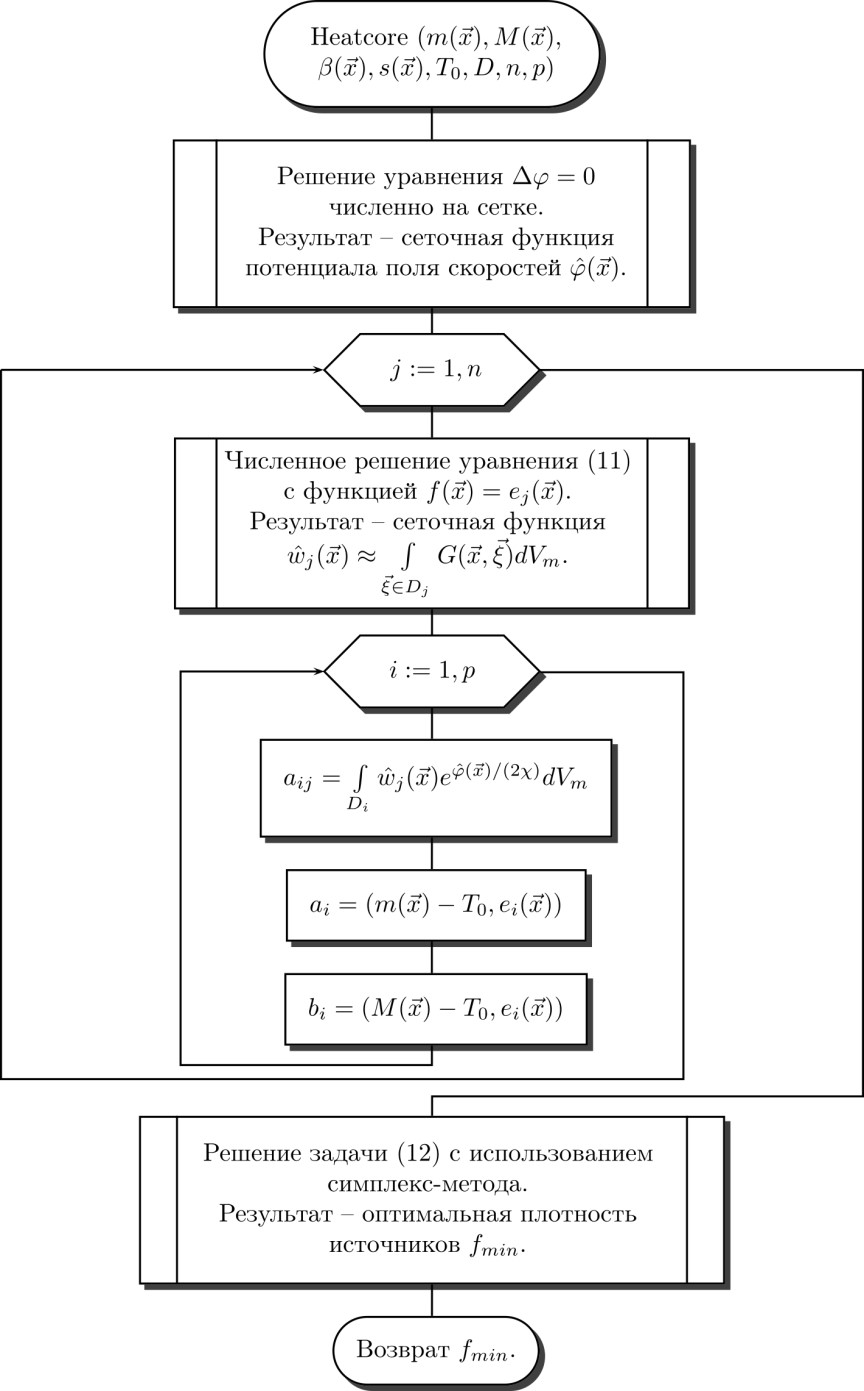
\includegraphics[width=7cm]{{pictures/picturefile_9_1}}
		\caption*{ Рис. Д.1. Блок-схема алгоритма для решения m-мерной задачи }
 	 \label{picture_9_1}
	\end{center}
\end{figure}




%\ref{ picture_4_2 }




В дальнейшем считается, что ячейки возникают в результате разрезания области $D$ точками ($m{=}1$), двумя семействами параллельных сторонам D прямых ($m{=}2$) или тремя аналогичными семействами плоскостей ($m{=}3$). На рис. Д.1 приведена блок-схема алгоритма решения $m$-мерной задачи для движущейся среды с использованием численного метода нахождения обменной матрицы. Для неподвижной среды блок-схема аналогична, но не содержит блока нахождения потенциала поля скоростей. На рис. Д.2 и Д.3 приведены графики стабилизации значений $(J_n)_{min}$ с ростом $n$, полученные в результате численных экспериментов в трехмерном случае, соответственно для неподвижной и движущейся сред с различными значениями  $\chi$.




\begin{figure}[h!]
	\begin{center}
		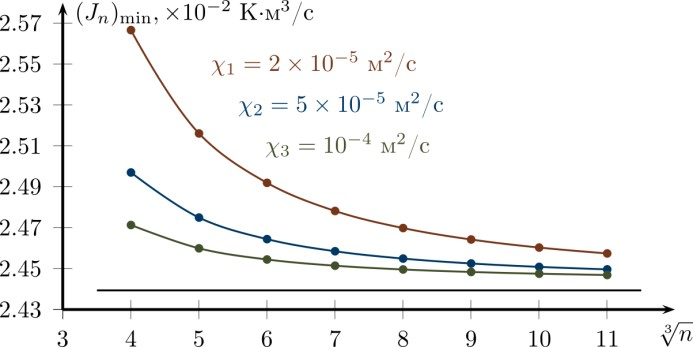
\includegraphics[width=7cm]{{pictures/picturefile_9_2}}
		\caption*{ Рис. Д.2. Зависимость значения $(J_n)_{min}$ от $n$ для неподвижной среды }
 	 \label{picture_9_2}
	\end{center}
\end{figure}







\begin{figure}[h!]
	\begin{center}
		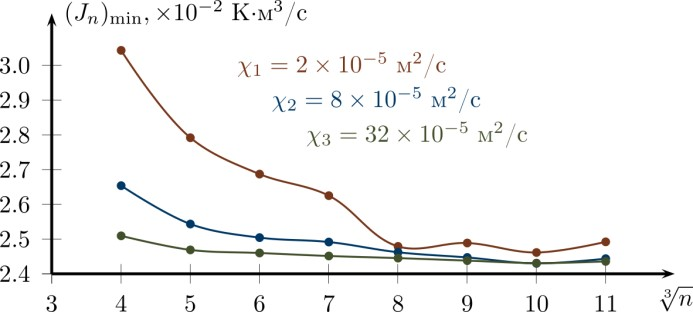
\includegraphics[width=7cm]{{pictures/picturefile_9_3}}
		\caption*{ Рис. Д.3. Зависимость значения $(J_n)_{min}$ от $n$ для движущейся среды }
 	 \label{picture_9_3}
	\end{center}
\end{figure}






На рис. Д.4 приведён результат численного эксперимента для
3-мерной области D размером $5 \times 4 \times 3$ м с принудительным источником холода. В качестве вещества, заполняющего область, был выбран воздух с коэффициентом температуропроводности $\chi{=} 2,216\times10^{-5} $  м$^2$/с. Границы области выполнены из кирпича с коэффициентом температуропроводности  $\chi_\kappa{=} 5,2\times10^{-7} $  м$^2$/с толщиной 30 см. На дальней плоскости имеется окно с  $\chi_c{=} 3,4\times10^{-7} $  м$^2$/с площадью 3м$^2$ (стеклянное окно). В правую грань области входит вещество со скоростью $s_2(x,y,z) {=} 10^{-4}$ м/с ($Г_+$ имеет площадь 2м$^2$). Симметрично с левой стороны имеется участок стока $Г_-$ такой же площади с такой же скоростью вещества $s_1(x,y,z) {=} 10^{-4}$ м/с. Минимальный и максимальный профили температур заданы функциями $m(x,y,z) {=} 290 $K, $M(x,y,z) {=} 320 $K, температура внешней среды $T_0 {=} 260 $K. Область контроля занимает всю область за исключением пространства вблизи входа воздуха $Г_+$ \[\tilde{D}{=}D-\{x>4,5\:и\:z>0,5\:и\:z<2,5\}.\]





\begin{figure}[h!]
	\begin{center}
		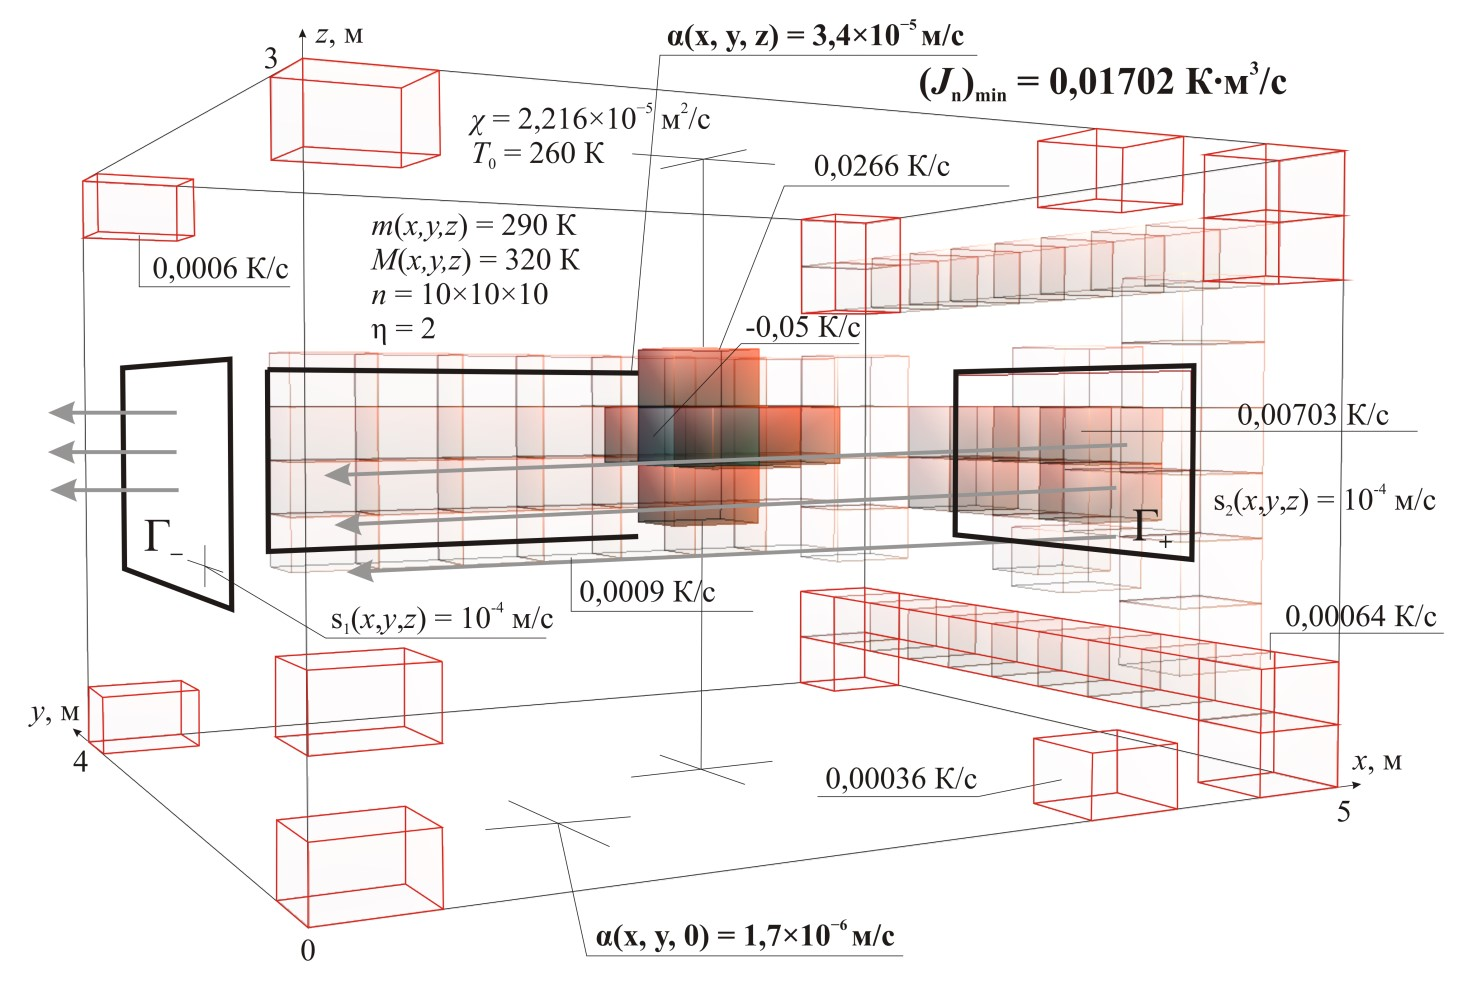
\includegraphics[width=7cm]{{pictures/picturefile_9_4}}
		\caption*{ Рис. Д.4. Оптимальное расположение источников тепла внутри параллелепипеда  }
 	 \label{picture_9_4}
	\end{center}
\end{figure}





Разноцветными объёмами показана искомая оптимальная плотность источников тепла (красные) и сток (синий). Источники распределяются вблизи места входа вещества, вдоль окна, а также около стока, таким образом его нейтрализуя. Суммарная  интенсивность источников имеет значение 0,01702\: К $\cdot$ $\text{м}^3$/с. Для перевода в систему СИ необходимо вычислить потери тепла в единицу времени(Дж/с) через границу
$$J_1 = \int\limits_{\Gamma_0}\frac{\chi_1}{d}u(x,y,z)dS+\int\limits_{\Gamma_-}\frac{(\chi_1)_{\text{в}}}{\chi}s_1(x,y,z)u(x,y,z)dS,$$
где $\chi_1$ --  коэффициент теплопроводности через границу во внешнюю среду [Вт/(м$\cdot$К)], $d$ – толщина стенки. Для стекла $(\chi_1)_c= 1 \text{Вт/(м}\cdot \text{К})$, кирпича $(\chi_1)_{\text{к}} = $ 0,5 Вт/(м$\cdot$К), воздуха $(\chi_1)_{\text{в}}$ = 0,0243 Вт/(м$\cdot$К). Результирующее значение $J_1{=}13\:131$\:Вт.

Для проверки эффективности был проведён следующий эксперимент. Было взято некоторое случайное распределение источников (рис. Д.5) и решена прямая задача теплопроводности для той же самой области (рис. Д.4) и тех же параметрах среды, но без стока тепла. В результате было получено, что случайное распределение источников нагревает область контроля в диапазоне температур $292{,}8{-}364{,}8\:$K. Затем была решена прямая задача с $m(x,y,z){=}292{,}8\:$K и $M(x,y,z){=}364{,}8\:$K при $(x,y,z){\subseteq}\tilde D$. В итоге получилось, что случайное распределение (рис. Д.5) имеет суммарную интенсивность $0,02687\:$К $\cdot$ $\text{м}^3$/с, а оптимальное (рис. Д.6) – $0,01476\:$К $\cdot$ $\text{м}^3$/с. Сэкономленная мощность при этом составляет около 45\%.

\begin{figure}[h!]
	\begin{center}
		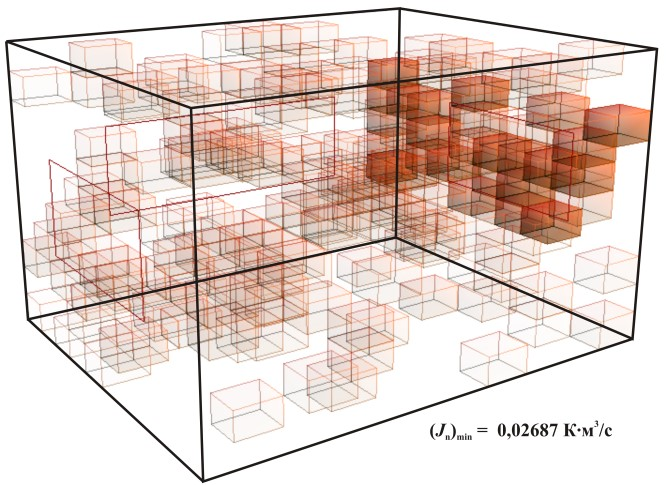
\includegraphics[width=7cm]{{pictures/picturefile_9_5}}
	\center{	\caption*{ Рис. Д.5. Случайное расположение источников тепла внутри параллелепипеда  }}
 	 \label{picture_9_5}
	\end{center}
\end{figure}




\begin{figure}[h!]
	\begin{center}
		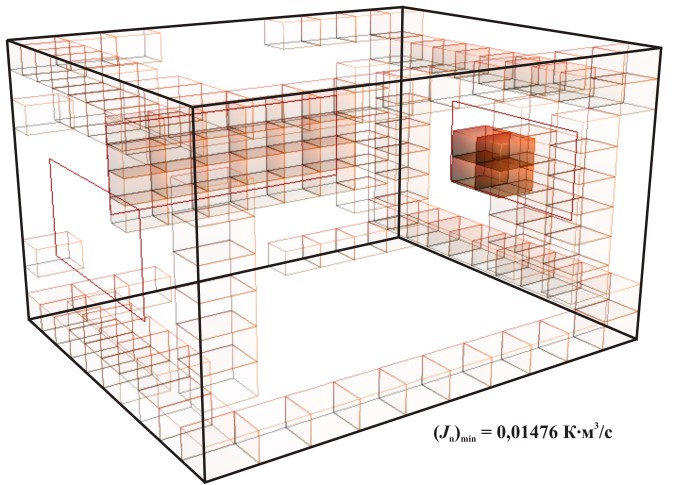
\includegraphics[width=7cm]{{pictures/picturefile_9_6}}
		\caption*{ Рис. Д.6. Оптимальное расположение источников  внутри параллелепипеда   }
 	 \label{picture_9_6}
	\end{center}
\end{figure}



На рисунке Д.7 представлен результат расчёта оптимального распределения источников тепла внутри области сложной геометрической формы размером $5 \times 3,5 \times 10$ м, составленной из тетраэдров в программе Solidworks. Большая часть границы области выполнена из материала с коэффициентом теплопередачи $\alpha_1{=}4\:\text{Вт}(\text{м}^2{\cdot}\text{К})$, за исключением небольшого окна с $\alpha_2{=}0,5\:\text{Вт}(\text{м}^2{\cdot}\text{К})$. Область заполнена воздухом с коэффициентом теплопроводности  $\chi{=} 0,0267\: \text{Вт}(\text{м}{\cdot}\text{К})$. До решения задачи оптимизации в область было добавлено $n{=}544$ источника тепла таким образом, чтобы они полностью заполнили область $D$ (за исключением промежутков между источниками). Область контроля температуры $\tilde D$, температура внешней среды и температурный коридор были заданы следующими:\[\tilde{D}=\Bigl\{(x-2,5)^2+(y-1)^2<2,2^2\Bigr\}\cup\{z<1\},\]
        \begin{equation*}
        m(x,y,z)=
        \begin{cases}
        5^oC,\:z>1,\\
        25^oC,\:z\le 1,
        \end{cases}
        M(x,y,z)=80^oC,\quad T_0=0^oC
        \end{equation*}



\begin{figure}[h!]
	\begin{center}
		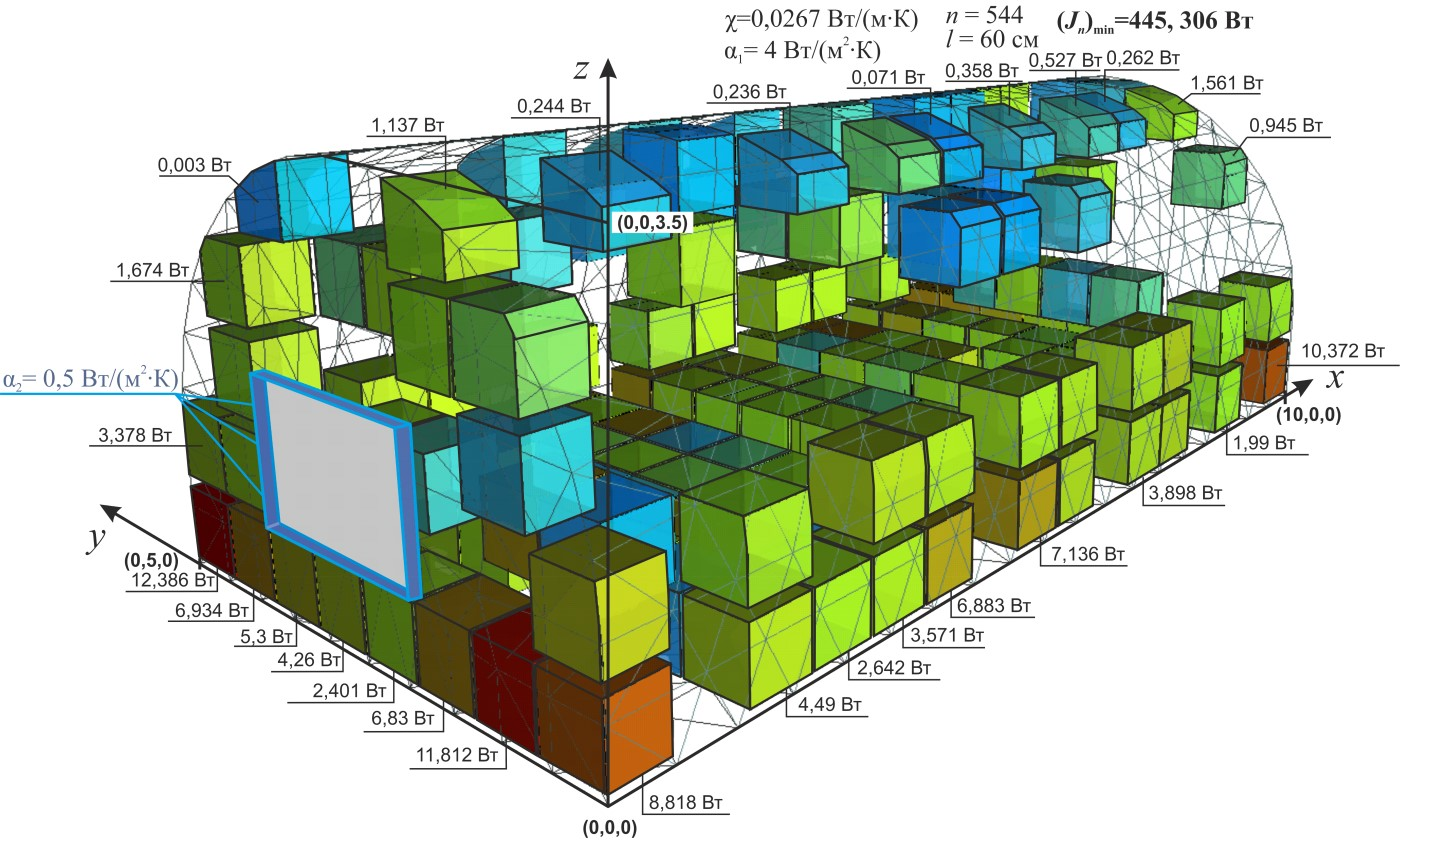
\includegraphics[width=7cm]{{pictures/picturefile_9_7}}
		\caption*{ Рис. Д.7: Оптимальное расположение источников тепла при $D=D_f$   }
 	 \label{picture_9_7}
	\end{center}
\end{figure}




На рис. Д.7 оптимальное распределение источников показано в виде объёмов различного цвета. Источники красного оттенка являются самыми мощными, зелёного – средней мощности, синего – малой мощности. Некоторые источники имеют нулевую мощность, т.е. отсутствуют, и на рисунке не показаны. Источники стабилизируются в основном вдоль границы области. Это объясняется тем, что необходимо компенсировать рассеивание тепла через границу, которая имеет сравнительно большой коэффициент теплопередачи, и обеспечить около неё температурный коридор. Самые мощные источники располагаются на углах, так как здесь самое большое рассеивание тепла. По условию эксперимента, верхнюю часть области $(z{>}1)$ нужно нагреть только до температуры $5^0\text{C}$, поэтому алгоритм располагает в данной части только источники малой мощности. Суммарная мощность источников тепла составляет $(J_n)_{min}{=}445,306\;\text{Вт}$. Исходная сетка содержала 6487 тетраэдров. После модификации сетки и добавления источников тепла количество многогранников увеличилось до 67912.

\textbf{Выводы.}Регулярность конечномерной аппроксимации $Z_0(n)$ по функционалу показывает лишь принципиальную возможность приближенного нахождения квазирешения. Остается открытым вопрос о том насколько большим нужно взять $n$, чтобы получить квазирешение с данным допуском $\varepsilon$. Из приведенных результатов вычислений видно, что последовательность $(J_n)_{min}$ довольно быстро стабилизируется с ростом $n$. Для случая неподвижной среды удается довольно близко подобраться к величине правой части оценки (\ref{equation_9_7}). Скорость стабилизации $(J_n)_{min}$ увеличивается с ростом температуропроводности среды $\chi$. Значения $(J_n)_{min}$ при больших $n$ слабо зависят от $\chi$ для неподвижной среды. Для движущейся среды эта зависимость значительно сильнее. Наконец, вычислительные эксперименты показывают возможность значительной экономии энергии в результате оптимизации по сравнению со случайной плотностью источников при таком же температурном коридоре.

\newpage
\subsection*{Заключение}

Завершая настоящее пособие, отметим, что в нем мы, в основном, рассматривали традиционные методы оптимизации. В настоящее время иногда успешно используют так называемые эволюционные методы и алгоритмы, в частности генетические алгоритмы. Все они моделируют базовые положения теории биологической эволюции – процессы отбора, мутации и воспроизводства. Здесь мы этих методов не касаемся, поскольку они относятся скорее к области искусственного интеллекта, а не к традиционным методам оптимизации. Подробно ознакомиться с эволюционными методами оптимизации можно по монографии \cite{literature_gladkov}.
